%%%%%%%%%%%%%%%%%%%%%%%%%%%%%%%%%%%%%%%%%
% University Assignment Title Page 
% LaTeX Template
% Version 1.0 (27/12/12)
%
% This template has been downloaded from:
% http://www.LaTeXTemplates.com
%
% Original author:
% WikiBooks (http://en.wikibooks.org/wiki/LaTeX/Title_Creation)
%
% License:
% CC BY-NC-SA 3.0 (http://creativecommons.org/licenses/by-nc-sa/3.0/)
% 
% Instructions for using this template:
% This title page is capable of being compiled as is. This is not useful for 
% including it in another document. To do this, you have two options: 
%
% 1) Copy/paste everything between \begin{document} and \end{document} 
% starting at \begin{titlepage} and paste this into another LaTeX file where you 
% want your title page.
% OR
% 2) Remove everything outside the \begin{titlepage} and \end{titlepage} and 
% move this file to the same directory as the LaTeX file you wish to add it to. 
% Then add \input{./title_page_1.tex} to your LaTeX file where you want your
% title page.
%
%%%%%%%%%%%%%%%%%%%%%%%%%%%%%%%%%%%%%%%%%

%----------------------------------------------------------------------------------------
%	PACKAGES AND OTHER DOCUMENT CONFIGURATIONS
%----------------------------------------------------------------------------------------

\documentclass[11pt]{article}
\usepackage[margin=1.0in]{geometry}
\usepackage{graphicx}
\usepackage{caption}
\usepackage{subcaption}
\usepackage{float}
\usepackage{url}
\DeclareGraphicsExtensions{.png}
\begin{document}

\begin{titlepage}

\newcommand{\HRule}{\rule{\linewidth}{0.5mm}} % Defines a new command for the horizontal lines, change thickness here

\center % Center everything on the page
 
%----------------------------------------------------------------------------------------
%	HEADING SECTIONS
%----------------------------------------------------------------------------------------

\textsc{\LARGE Wright State University}\\[1.5cm] % Name of your university/college
\textsc{\Large CS 7900}\\[0.5cm] % Major heading such as course name
\textsc{\large Final Report}\\[0.5cm] % Minor heading such as course title

%----------------------------------------------------------------------------------------
%	TITLE SECTION
%----------------------------------------------------------------------------------------

\HRule \\[0.4cm]
{ \huge \bfseries A Sentiment Analysis Application for Tweets}\\[0.4cm] % Title of your document
\HRule \\[1.5cm]
 
%----------------------------------------------------------------------------------------
%	AUTHOR SECTION
%----------------------------------------------------------------------------------------

\begin{minipage}{0.4\textwidth}
\begin{flushleft} \large
\emph{Author:}\\
Daniel \textsc{McIntyre} U00653482 % Your name

Nathan \textsc{Rude} U00637118% Your name

\end{flushleft}
\end{minipage}
~
\begin{minipage}{0.4\textwidth}
\begin{flushright} \large
\emph{Supervisor:} \\
Dr. Tanvi \textsc{Banerjee} % Supervisor's Name
\end{flushright}
\end{minipage}\\[4cm]

% If you don't want a supervisor, uncomment the two lines below and remove the section above
%\Large \emph{Author:}\\
%John \textsc{Smith}\\[3cm] % Your name

%----------------------------------------------------------------------------------------
%	DATE SECTION
%----------------------------------------------------------------------------------------

{\large \today}\\[3cm] % Date, change the \today to a set date if you want to be precise

%----------------------------------------------------------------------------------------
%	LOGO SECTION
%----------------------------------------------------------------------------------------

%\includegraphics{Logo}\\[1cm] % Include a department/university logo - this will require the graphicx package
 
%----------------------------------------------------------------------------------------

\vfill % Fill the rest of the page with whitespace

\end{titlepage}
%--------------------------------------
%  Content Sections
%------------------------------------

\section{Goal}
Social media is a very ingrained component of our culture. In this day and age, there are social media users all over the world. In fact, social data is a very rich source of data in today’s information age. For this project, we aim to leverage the power of social data from Twitter. As a micro-blogging outlet, users regularly churn out bite-sized chunks of information that can be analysed for information on just about any topic. By aggregating tweets about a certain topic from Twitter, one can get a general sentiment from the populous about that certain topic. 

Since tweets can be retrieved in real time, the sentiment of current and trending topics, such as presidential debates and debate topics, can be evaluated to determine how the populous feels about each topic. Understanding and incorporating this user feedback, specifically by examining tweets with a negative sentiment, one can receive the feedback required to move towards a more popular opinion.

\section{Objective}
We created a web application that allows users to view the sentiment of topics on Twitter. Through the use of two API’s, we 1) retrieved tweets from Twitter and 2) performed sentiment analysis on these tweets and also aggregated the general sentiment about a topic. 

\section{Approach}
This application can be split into two parts: a frontend for the user to select topics and view the sentiment, and a backend for the text retrieval and sentiment analysis to take place. 

\subsection{Frontend}
The user interface was developed with HTML, CSS and Javascript, technologies that have been learned in class. Specifically we used nodejs as a server backend to host the site. We used the Express framework for routing and logic as well as Swig for the user interface templating language. Swig provided a flexible design that incorporated template inheritance and ease of use. In addition to Swig, Bootstrap was used for the CSS styling. 

The user interface is comprised of two parts, the user input section, and the  the results display. The user input section consists of a start date, end date, topic search, and a selection to search by topic or by tweet id. The start and end dates define the time range that returned results will occur in. The topic search input can be a tweet topic, or can be a tweet id. If the tweet id check mark is selected, a specific tweet with the specified id will be searched and if found, it's sentiment will be analysed. The tweet results section shows the tweet, the tweet sentiment and the person who tweeted it. The accumulated tweet sentiment is also displayed to the user. 

Using these technologies we can create a dynamic layout that, given a search topic, can display several retrieved tweets with their individual sentiment, as well as the overall sentiment of a topic.

\subsection{Backend}
The backend was split into two parts: tweet retrieval and text sentiment. 

\subsubsection{Tweet Retrieval}
The tweet retrieval was performed with the node module {\em twit}. This module allowed us to search twitter with query strings that encode the topic, start and end date. Using this API we can also search twitter with a specific tweet id to get the associated tweet. The twitter API does have its drawbacks however. The first drawback being that there is a usage rate limit for the search API of 180 calls per 15 minutes. 

The second limitation is the page size when using the search API. The page size denotes the number of tweets retrieved per api call up to a maximum of 100 tweets. This allows us to retrieve 100 tweets with each 180 allowed API calls for a total of 18,000 tweets each 15 minutes. This might seem like a large number, however this number can be easily exhausted when querying a popular topic. For example, querying "Trump" will return 100 results within a time window of a few seconds. Querying another, less popular topic such as "Grand Canyon" will return 100 tweets within a time window of several hours (note that this is situational and the frequency of requests could change).

The third limitation is that the search API only indexes tweets within a 7 day window of when they were created. After roughly 7 days, the tweets are removed from the search index and are unable to be retrieved. This makes it impossible to retrieve tweets by topic that are further in the past.

To accommodate all of these limitations, our program only returns 100 tweets per search. However calculating the sentiment of only 100 tweets is not indicative of the overall sentiment of a topic. For popular topics that are constantly being discussed, this 100 tweet limit is a mere snapshot of a few seconds of conversation. The only way to overcome these limitations would be to use the Twitter streaming API to retrieve tweets as they occur, however there are no current plans to integrate this into our application.

\subsubsection{Text Sentiment}
The sentiment analysis was performed with the node module {\em retext-sentiment} which is a plugin for the retext module. The retext-sentiment module operates at the sentence level through the word level. Each word is assigned a polarity and negation is also supported. The word "bad" would have a negative connotation, but the phrase "not bad" would not have a negative connotation. There is also built in support for emoji as well. A smiley will have a positive connotation while a frown would have a negative connotation. 

The overall sentiment of a tweet would be {\em sentiment = good words - bad words}. This gives us a sentiment polarity that represents how positive or negative the sentiment is and, consequently, a valence of negative, neutral or positive.

One limitation of this module is that it uses a mapping of sentiment to words, so if a word is misspelled, the sentiment cannot be computed. Since this module is used on unprocessed twitter data, there is the possibility that tweets exhibiting a negative sentiment, but are not spelled correctly, will not be labelled accurately.

\section{Evaluation}
To evaluate the sentiment analysis component of the application we used the following two sub-datasets from the Sentiment Strength Twitter Dataset (SS-Tweet) \cite{saif2013evaluation}: 1) Youtube comments and 2) twitter tweets (see Table \ref{tab:cdescr}). Using data from two domains allowed us to better evaluate the robustness of our sentiment analysis tool. 

To keep the evaluation simple, we performed binary evaluation for this multiclass problem. 
The testing datasets were labeled with a mean positive and mean negative value for each sample. To calculate the sentiment, we define {\em sentiment = good - bad} and then threshold it into a class {\em negative, neutral, positive} based on it's value.
To compute precision and recall for a multiclass problem, we transformed the problem into several one-vs-many problems, calculated the precision and recall for those, and then took the average values for the multiclass problem.

\begin{table}[!ht]
\centering
\begin{tabular}{|c|c|c|c|c|} \hline
\textbf{Dataset} & \textbf{Samples} & \textbf{Positive} & \textbf{Neutral} &\textbf{Negative} \\ \hline \hline
Twitter & 4,242 & 1,340 & 1,953 & 949 \\ \hline
Youtube & 3,307 & 1,665 & 875 & 767 \\ \hline
\end{tabular}
\caption{Dataset class breakdown}
\label{tab:cdescr}
\end{table}

The results of the sentiment analysis evaluation can be seen in Table \ref{tab:smetric} and Figure \ref{fig:confmat}. We can see that the Twitter and Youtube datasets have similar precision and recall values, and this implies that this sentiment module is robust across different text domains.
Now while the precision and recall values do not seem that high, it's important to realize that not even humans can accurately determine the sentiment of a text 100\% of the time. In fact humans can only determine the correct sentiment 70-80\% \cite{sent2}\cite{sent1}\cite{mashable} of the time! This is because humans do not universally agree with each other on any subjective matter.

Examining the confusion matricies in Figure \ref{fig:confmat} we can see that the algorithm mostly has trouble with the neutral class. With sentiment being such a subjective issue, it intuitively makes sense that there would be more trouble evaluating whether a text is {\em positive vs neutral} or {\em negative vs neutral}. The lines can be more gray here rather than the stark contrast that a {\em positive vs negative} tweet would have. 

\begin{table}[!ht]
\centering
\begin{tabular}{|c|c|c|} \hline
\textbf{Dataset} & \textbf{Precision} & \textbf{Recall} \\ \hline \hline
Twitter & .55 & .58  \\ \hline
Youtube & .53 & .55 \\ \hline 
\end{tabular}
\caption{Sentiment Metrics}
\label{tab:smetric}
\end{table}

\begin{figure}[t!]
    \centering
    \begin{subfigure}[b]{0.4\textwidth}
            \centering
            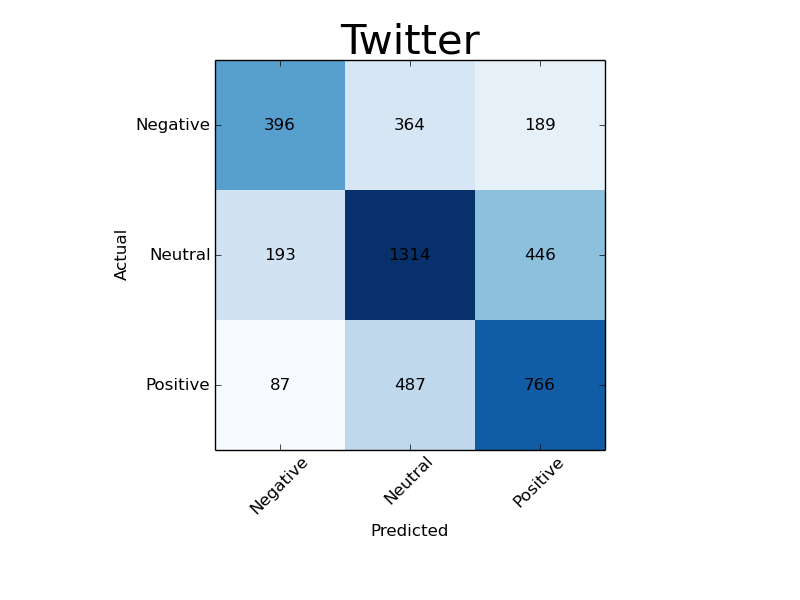
\includegraphics[width=\textwidth]{fig/Twitter.png}
            \caption{}
            \label{fig:twitter}
    \end{subfigure}
    \begin{subfigure}[b]{0.4\textwidth}
            \centering
            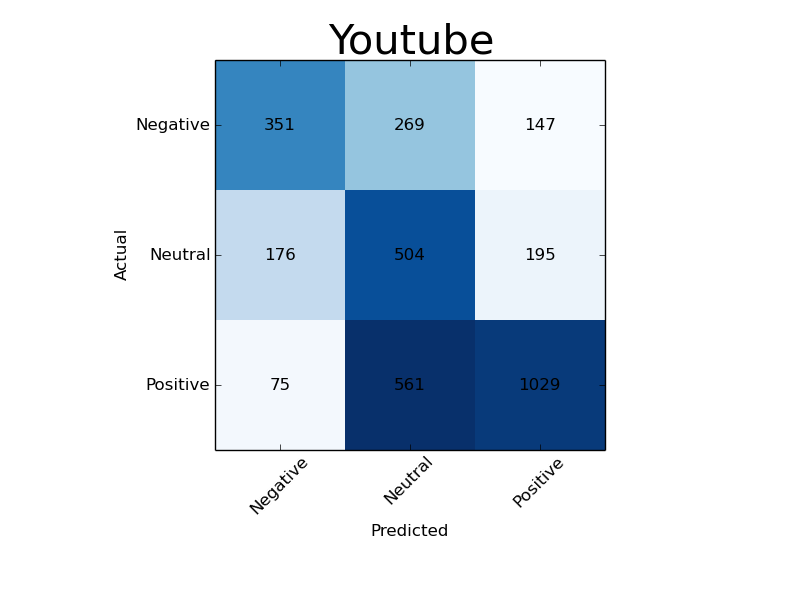
\includegraphics[width=\textwidth]{fig/Youtube.png}
            \caption{}
            \label{fig:youtube}
    \end{subfigure}
    \caption{Sentiment Confusion Matrices}
    \label{fig:confmat}
\end{figure}

Since the algorithms performs much better than just guessing the class (which would be a 33.3\% precision), we conclude that the performance of this algorithm is adequate for the task at hand.

\section{Results}
put sample queries here and evaluate and analyze the results

1) gender neutral bathrooms
 
\section{Conclusion}
\pagebreak

\bibliography{egbib}
\bibliographystyle{plain}

\end{document}